% !TEX root=index.tex
\chapter{Il Vehicle Routing Problem}\label{ch:vrp}

Il \emph{Vehicle Routing Problem} (VRP) è un tipico problema legato alle reti di distribuzione che generalizza il \emph{Traveling Salesman Problem} (problema del commesso viaggiatore, in breve TSP). Dati un insieme di clienti distribuiti all’interno di una rete di trasporto ed una flotta di veicoli, l’obiettivo del problema è quello di determinare il percorso ottimo di ciascun veicolo adibito alla distribuzione al fine di soddisfare le richieste di ciascun cliente.

Il set di percorsi relativi ai veicoli, che di qui in avanti chiameremo \emph{rotte}, deve essere ricercato nell’ottica dell’ottimizzazione di una certa funzione obiettivo, che varia a seconda dell’applicazione: i problemi di \emph{vehicle routing} sono solitamente problemi di minimizzazione, il cui scopo è quello di contenere il più possibile la lunghezza complessiva delle rotte o, più generalmente, il costo totale della distribuzione.

Nella ricerca del set ottimo occorre tenere in considerazione le caratteristiche della flotta dei veicoli e dei clienti. Si possono identificare varie sottoclassi di problemi di VRP a partire dalla classificazione di tali caratteristiche: di seguito ne presenteremo alcune tra le più significative.

Nella sua formulazione più basilare, un problema VRP vede la presenza di un deposito centrale da cui parte una flotta di veicoli\footnote{Per flotta di veicoli si intende un insieme costituito da due o più veicoli. Si tenga presente che, un problema VRP in cui si ha a disposizione un solo veicolo degenera immediatamente in un problema TSP.}, il cui compito consiste nella \emph{distribuzione di un bene} ad una serie di clienti che ne fanno richiesta. Ogni cliente della rete è caratterizzato dalla \emph{quantità di tale bene di cui fa richiesta} al distributore. Ciascun veicolo della flotta, dopo aver terminato il suo giro di consegne, deve far ritorno al deposito.

Non vengono posti limiti alle quantità di bene trasportabili da ciascun veicolo, il che rende poco adatta questa iniziale formulazione ad una reale applicazione in un problema di distribuzione. Vincolando la capacità massima di ciascun veicolo, si ottiene la prima variante al VRP, chiamata \emph{Capacitated Vehicle Routing Problem}, in breve CVRP.

Nei problemi di CVRP viene quindi imposto che ogni veicolo della flotta non può trasportare più di una determinata quantità del bene, il cui valore è stabilito dalle limitazioni fisiche del veicolo stesso.

In altre parole, dovendo ciascun veicolo servire il sottoinsieme dei clienti presenti sulla rotta ad esso assegnata, la \emph{quantità del bene complessiva, richiesta da tali clienti, non dovrà superare la capacità di carico del veicolo stesso}.

In un caso reale, inoltre, potrebbe essere necessario imporre delle condizioni relativamente all’orario entro cui il veicolo deve giungere dal cliente. Si pensi, ad esempio, alle consegne che un fornitore deve effettuare ad un cliente che si occupa di vendita al dettaglio. È naturale assumere che le consegne debbano essere effettuate come minimo entro l’orario d’apertura. Altre volte i clienti possono stabilire un preciso intervallo orario entro cui sono disposti a ricevere la merce.

Questo tipo di limitazioni prende il nome di \emph{time window} e costituiscono degli intervalli orari, definiti da ciascun cliente, entro i quali devono essere effettuate le consegne. Questo tipo di problemi costituisce una sottoclasse del VRP e prende il nome di \emph{Vehicle Routing Problem with Time Windows} (VRPTW).

Altre varianti degne di nota di problemi di \emph{vehicle routing} sono le seguenti:
\begin{description}
	\item[VRPPD] acronimo di \emph{Vehicle Routing Problem with Pickup and Delivery}. Definite quantità di un bene devono essere prelevate non dal deposito centrale, ma da un insieme di punti di raccolta distribuiti sulla rete logistica, e devono essere consegnate ad un insieme di clienti.

	\item[VRPMT] ovvero \emph{Vehicle Routing Problem with Multiple Trips}. Ad ogni veicolo viene assegnata più di una rotta da seguire, al termine di ognuna delle quali deve tornare al deposito per ricevere un nuovo carico.

	\item[OVRP] \emph{Open Vehicle Routing Problem}. I veicoli della flotta in questa categoria di problemi non devono ritornare al deposito una volta concluso il giro di consegne.
\end{description}

Nella maggior parte dei casi reali, i problemi di distribuzione possono essere ricondotti alle classi CVRP e VRPTW. 

La rete di distribuzione trova una naturale rappresentazione mediante l’utilizzo di un \emph{grafo completo} di cui il \emph{deposito} ed i \emph{clienti} ne costituiscono i nodi.
Ogni cliente \emph{i-esimo} è caratterizzato dalla quantità di bene richiesta, indicata con $q_i$, ed è disposto ad essere visitato dal veicolo per la distribuzione tra l’istante $a_i$ e l’istante $b_i$.
Per questioni esemplificative si assume che la flotta di veicoli sia omogenea e che questi ultimi non possano trasportare una quantità di bene superiore alla loro capacità massima $Q$.

\section{Accenni alla teoria dei grafi e delle reti} % (fold)
\label{sec:accenni_alla_teoria_dei_grafi_e_delle_reti}
	Di seguito si riportano alcuni concetti della Teoria dei grafi e delle reti che riteniamo utili per la corretta comprensione del modello che verrà analizzato nei capitoli successivi:

	\begin{itemize}
		\item Un \emph{grafo}, $G = (N, A)$, e una coppia di insiemi: $N$ è un insieme finito e non vuoto di elementi, mentre $A$ è un insieme finito di coppie di elementi distinti di $N$.
		$N$ è detto insieme dei \emph{nodi}, e usualmente viene indicato mediante i primi $n = |N|$ numeri naturali: $N = \{1 , 2 , \cdots , n \}$. L’insieme $A$, detto insieme degli \emph{archi}, è in generale indicato con $A = \{ a_1 , a_2 , \cdots , a_m \}$ ($m = |A|$). 
		Nel seguito un arco verrà indicato principalmente da una coppia di nodi $(i,j)$, piuttosto che dal nome $a_k$.
		\begin{figure}[H]
			\centering
			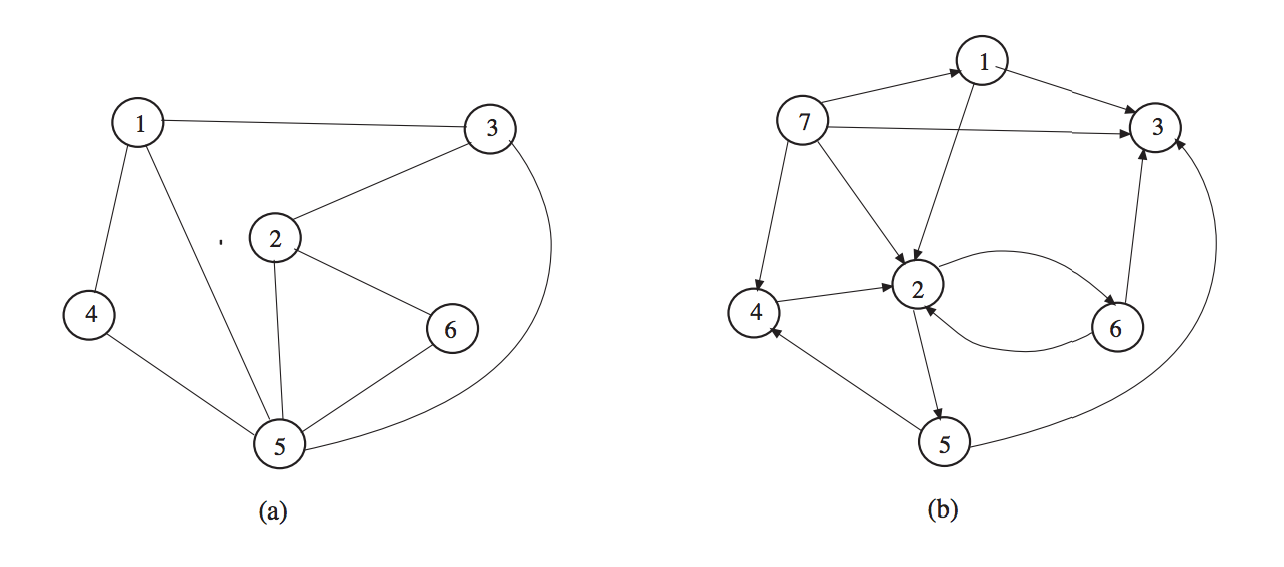
\includegraphics[keepaspectratio=true,scale=0.3]{img/esempio_grafi.png}
			\caption{Esempi di grafi}
			\label{fig:graph_example}
		\end{figure}

		\item Un grafo si definisce \emph{orientato} se tutti gli archi $(i,j) \in A$ sono orientati, ovvero le coppie $(i,j)$ sono ordinate; un grafo si definisce \emph{non orientato} o \emph{simmetrico} se tutti gli archi $(i,j) \in A$ non sono orientati. 
		Solitamente, per rimarcare la differenza tra i due casi, i nodi di un grafo simmetrico vengono chiamati \emph{vertici}, ed il grafo si indica con $G = (V,E)$, essendo $E$ l’insieme dei lati.Si definisce grafo \emph{completo} quello in cui esistono archi che connettono tra loro tutti i nodi.
		\begin{figure}[H]
			\centering
			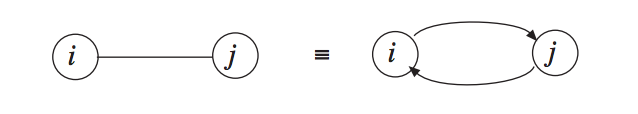
\includegraphics[keepaspectratio=true,scale=0.6]{img/equivalenza_archi.png}
			\caption{Equivalenza tra un arco non orientato ed una coppia di archi orientati}
			\label{fig:arc_equivalence}
		\end{figure}		

		\item Una \emph{rete} è un grafo ai cui nodi e/o archi sono associati dei pesi. Tali pesi possono avere significati diversi a seconda del contesto; ad esempio, nel caso del trasporto di merce da parte di un veicolo, i pesi associati agli archi possono rappresentare la distanza (in km) da un punto di consegna ad un altro, mentre i pesi associati ai nodi possono rappresentare la quantità di merce richiesta dal cliente.

		\item Dato un grafo orientato, si dice \emph{cammino} dal nodo $i_0$ al nodo $i_k$ una successione finita di archi $C = \left \{ (i_0, i_1),(i_1, i_2), \cdots (i_{k-1}, i_k) \right \}$ tale che il nodo terminale di un arco coincide con il nodo iniziale dell’arco successivo. Se $i_0 = i_k$, $C$ è detto un \emph{ciclo}.

		\item Un ciclo viene definito \emph{ciclo hamiltoniano} se passa \emph{per ogni nodo} del grafo una e una sola volta. Un ciclo senza ripetizione di archi formato da $m$ archi è detto \emph{ciclo euleriano}; esso passa attraverso \emph{ciascun arco} del grafo una e una sola volta. 
	\end{itemize}
% section accenni_alla_teoria_dei_grafi_e_delle_reti (end)